\section*{Dati e risultati}

\subsection*{Determinazione della capacità incognita}

In questa prima parte della relazione illustreremo come abbiamo trovato la capacità incognita ($C_3$) sfruttando le proprietà del circuito rappresentato in Figura \ref{fig:notch}.
Risolvendo questo tipo di circuito, nel caso in cui questo sia bilanciato, si ottengono i seguenti risultati:

%\begin{equation}
%	\frac{R_4}{R_3} \,+\, \frac{C_3}{C_4} \,=\, \frac{R_2}{R_1} \qquad \text{da cui si ottiene} \qquad C_3 \,=\, %\Bigl(\frac{R_2}{R_1} \,-\, \frac{R_4}{R_3}\Bigr)\cdot\,C_4
%	\label{eq:C}
%\end{equation}
\begin{equation}
	\omega^2\,R_3\,R_4\,C_3\,C_4 \,=\, 1 \qquad \text{da cui si ottiene} \qquad C_3 \,=\, \frac{1}{\omega^2\,R_3\,R_4\,C_4}
	\label{eq:C_imm}
\end{equation}

dove $R_3,\,R_4$ indicano le resistenze da $1\,\si{\kilo\ohm}$, $C_4$ è il valore della capacità nota ed infine $\omega$ non è altro che il valore del periodo dell'impulso, ovvero $\omega \,=\, 2\,\pi\,\nu_0$ dove $\nu_0$ indica la frequenza in ingresso del nostro circuito.

Quindi l'operazione fondamentale da fare al fine di sfruttare la relazione sopra citata è quella di bilanciare il circuito. Bilanciare il circuito non vuol dire altro che regolare i valori della frequenza in ingresso ($\nu_0$) e della resistenza variabile ($R_1$) in modo tale che la diffrenza di potenziale tra $V_2$ e $V_1$ sia nulla o quantomeno tendente a zero :D.

%I valori teorici $C\ped{3teo}$ da noi trovati, sfruttando le due formule precedenti (\ref{eq:C_imm}) e (\ref{eq:C_teo_imm}), per la capacità incognita sono i seguenti:  
Il valore teorico $C\ped{3teo}$ da noi trovato per la capacità incognita è il seguente:

%\begin{equation*}
%	C\ped{3teo} \,=\, XXX \qquad \text{sfruttando la rezione (\ref{eq:C})}
%\end{equation*}
\begin{equation}
	C\ped{3teo} \,=\, 2.9 \,\pm\, 0.2 \,\si{\nano\farad}  \qquad \text{sfruttando la relzione (\ref{eq:C_imm})}
	\label{eq:C_teo_imm}
\end{equation}
%2.972638538603707e-09
%2.1155093730419337e-10

Mentre il valore sperimentale di $C\ped{3exp}$ ottenuto grazie alla misura diretta col multimetro digitale è:

\begin{equation}
	C\ped{3exp} \,=\, 3.0 \,\pm\, 0.2 \,\si{\nano\farad}
	\label{eq:C_exp} 
\end{equation}

\subsection*{Ponte di Wien come filtro notch}

Vogliamo ora scoprire se sia possibie utilizzare il ponte di Wien come filtro notch. A tal fine è necessario apportate alcune modifiche strutturali al circuito. Tali cambiamenti sono illustrati in Figura \ref{fig:notch}.

Abbiamo studiato la funzione di trasferimento del circuito, cioè il rapporto $V\ped{out}/V\ped{in}$, sia dal punto di vista teorico che da quello sperimentale. Risolvendo il circuito si ottiene la $V\ped{out} = V_1 - V_2$, con relativa ampiezza e fase. Si è poi misurato, al variare della frequenza, l'ampiezza e la fase (rispetto a $V\ped{in}$) di $V\ped{out}$. O almeno avremmo dovuto misurare tale fase.

Durante l'esecuzione dell'esperienza abbiamo però sbagliato, misurando l'ampiezza corretta, ma la fase di $V_1$ invece che quella di $V\ped{out}$. Per rimediare abbiamo dovuto adottare un approccio ibrido, ricavando $V_1$ e $V_2$ e utilizzando i dati sperimentali misurati risalire alla fase di $V\ped{out}$. La misura è stata quindi molto indiretta, con conseguente perdita di risoluzione. Per le resistenze usate, che non sono state misurate col multimetro, abbiamo dovuto usare l'incertezza di targa, pari al 5\%. Per fortuna abbiamo misurato le capacità, che hanno un incertezza nominale del 20\%.

Il grafico in Figura \ref{fig:g} riporta i diagrammi di Bode del circuito.

\begin{SCfigure}
    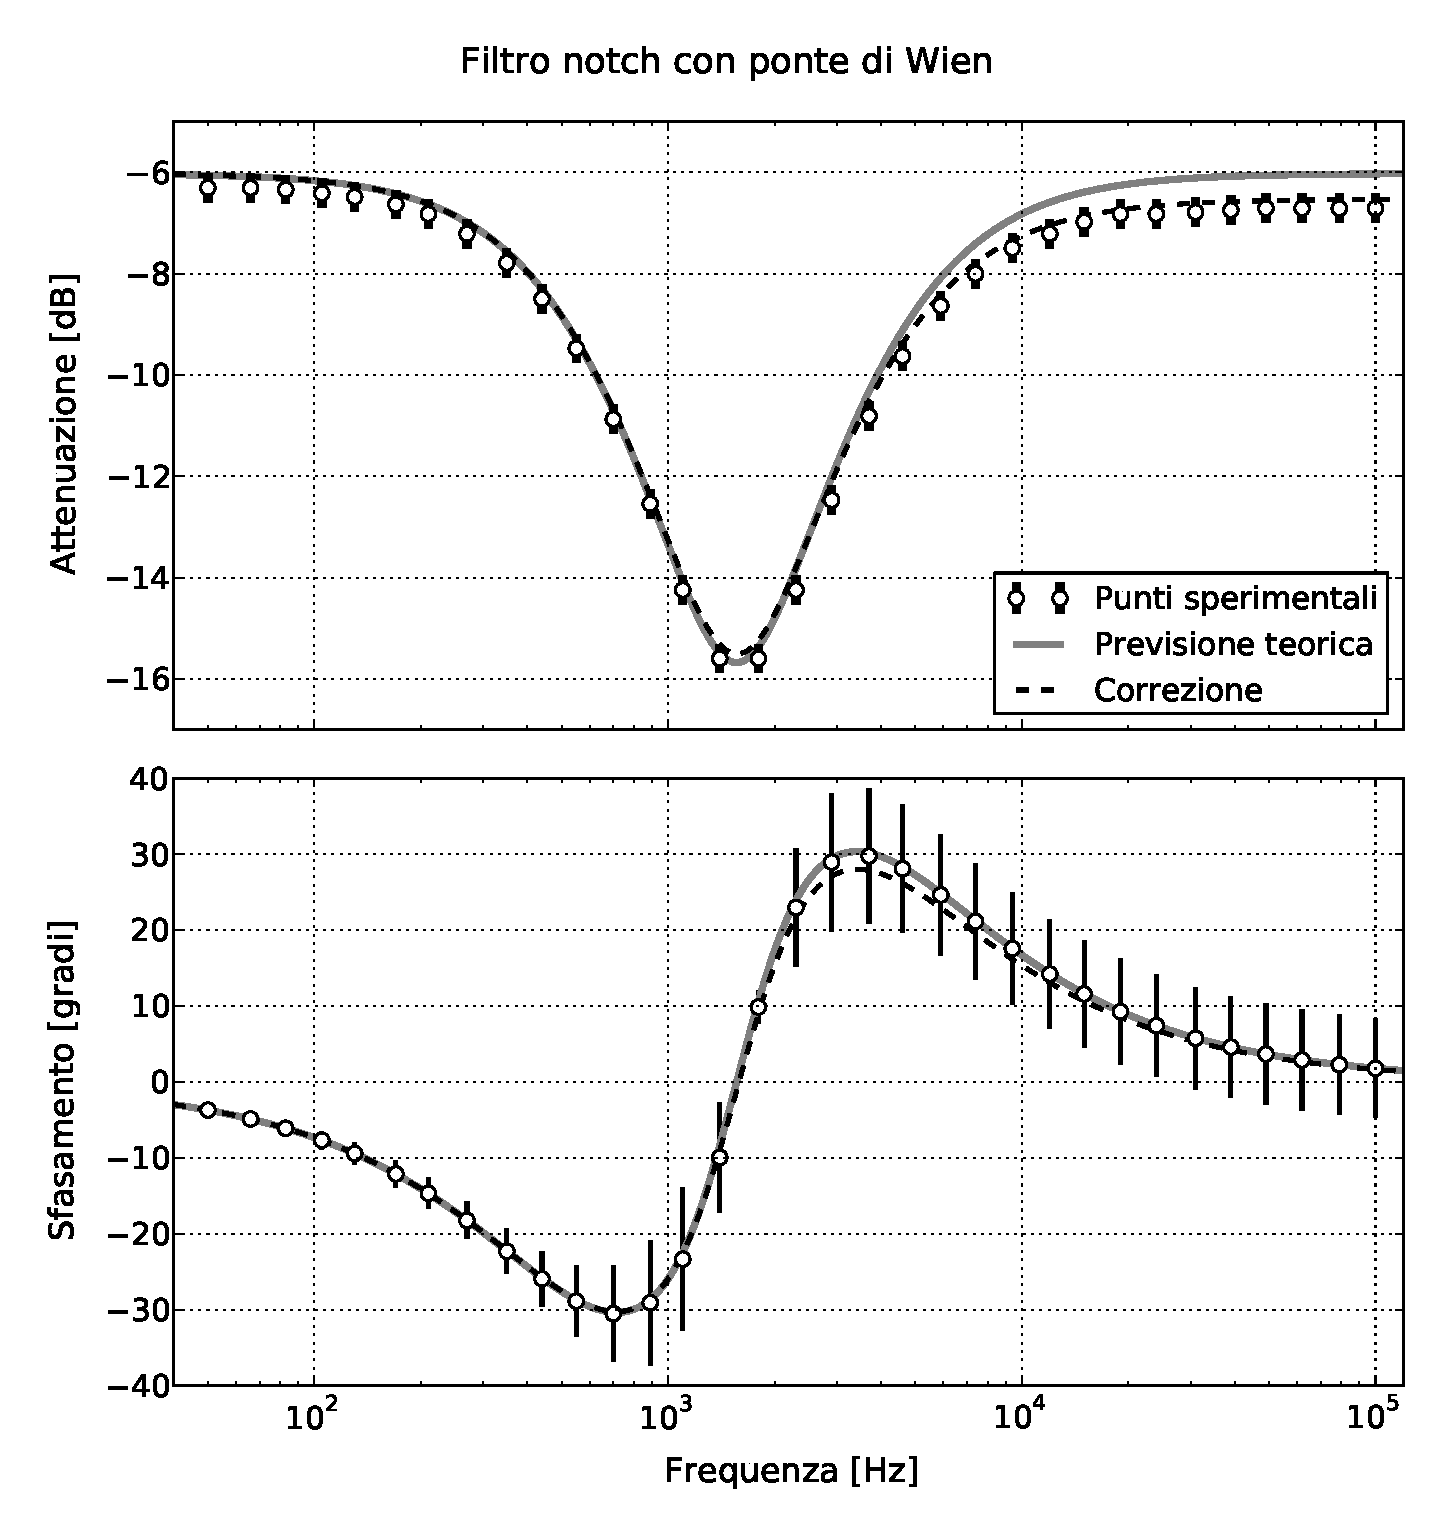
\includegraphics[scale=0.50]{g.pdf}
    \caption{Il grafico illustra i diagrammi di Bode per un filtro notch costruito con un
        ponte di Wien.
        I dati riguardano la tensione $V\ped{out} = V_1 - V_2$ in relazione a $V\ped{in}$. 
        Nel primo grafico i dati concordano con l'andamento previsto
        fino a circa 5 kHz. Abbiamo quindi corretto le nostre previsioni aggiungendo una resistenza
        in serie al condensatore $C_3$ (vedi Figura \ref{fig:notch}). Ad alte frequenze il
        condensatore si comporta come un corto circuito; è dunque necessario tenere in
        considerazione la resistenza dovuta al filo.
        La correzione è risultata molto consistente con i dati.
        Il secondo grafico mostra lo sfasamento di
        $V\ped{out}$ rispetto a $V\ped{in}$. Anche in questo caso i dati sono in accordo
        con la previsione teorica. Tuttavia vogliamo sottolineare che durante l'esperienza
        abbiamo misurato solo la fase di $V_1$ e l'ampiezza di $V\ped{out}$, a causa di un
        disguido. Abbiamo quindi dovuto estrapolare i lo sfasamento di $V\ped{out}$ utilizzando
        anche i valori delle resistenze, che non abbiamo misurato con il multimetro. Quindi
        i dati sono piagati da incertezze molto consistenti (per le resistenze
        abbiamo utilizzato il 5\%), come si nota dalle barre d'errore. 
    }
    \label{fig:g}
\end{SCfigure}
